
\chapter{Power System Simulation}\label{chap:powersys}

The purpose of this chapter is to test the feasibility and performance of the QDL method for the modeling and simulation of the dynamic performance of a relatively large and realistic power system model. The system model created for this evaluation is a three-phase network consisting of a synchronous machine, a turbine, a governor, an exciter, an induction motor, an ac/dc converter, a dc load, and a constant impedance load. All of these devices are connected through a three-phase network consisting of several buses and transmission lines. This study system contains a high range of transient behavior, from the slow mechanical transients of the rotating machines, to the very fast transients of the electrical quantities on the network. This is therefore mathematically a very stiff system model, which poses a challenge of effectively simulating the system over significant periods of simulation time while capturing the full range of transient behavior using a single representation of the power system. Because the QDL approach primarily quantizes the simulation states (and not time), it should therefore be well-suited to the task of simulating the slow and fast dynamics of system without some of the numerical stability and efficiency issues inherent in solving stiff systems using traditional time-slicing methods. 

The benefits of QDL methods are best leveraged by systems whose states have derivatives that approach zero at steady-state. A ac power system that has sinusoidal steady-state behavior in the stationary reference frame is therefore best modeled in the rotating reference frame using a Park transformation. The QDL method than then take advantage of the benefits of the QDL steady-state performance behavior. The variable time spans between state updates should be longer during steady-state conditions without sacrificing accuracy during the fast transients.

\section{System Model}

\begin{figure}[h]
    \label{fig:powersys}
    \centering
    \includegraphics[width=0.8\linewidth]{powersys.png}
    \caption{Power system schematic}
\end{figure}

The reference system is a three-phase, 60 Hz, 4160 V (line-line RMS) power system consisting of a synchronous machine being operated as a generator, connected to three loads via a network of buses and cables. An induction motor is connected to bus two and the other two loads, a dc load behind a converter and a constant impedance (RL) load are connected to bus three. The converter is represented as a non-linear dq averaged model. The cables are represented using a standard pi model. With 32 states, this power system is designed to be simple enough for the testing of a novel simulation method, while complex enough to represent a realistic, non-linear power system. For each device, a model was QDL compliant device model was formulated. These models are described in the next section.

The descriptions for each of the device models for the study system are given below, along with the derivation of the QDL model.

\section{Cable Model}

\begin{figure}[h]
    \label{fig:powersys_cable}
    \centering
    \includegraphics[width=0.75\linewidth]{powersys_cable.png}
    \caption{Cable model}
\end{figure}

Each cable is represented as a lumped pi model of a transmission line as described in \cite{gholizadeh2021}. The equivalent circuit is shown in figure \ref{fig:powersys_cable}. Note that only the q-axis model is shown. The d-axis portion of model and is identical to q-axis portion, except the voltage and current quantities are their d-axis counterparts. This model differs from the cable model in \cite{gholizadeh2021}, in that the shunt conductance and capacitance elements have been added to the ends of the branch in order to provide full latency required by the QDL and simulation method. This model provides full branch and node latency by exploiting the inherit latency from the physical branch inductance and the node capacitance. The dynamic equations that describe the cable model are 

\begin{equation} \label{eq:cable_iq}
\frac{d}{dt}i_{q}=\frac{-(R+\omega L)i_{q}+(v_{q1}-v_{q2})}{L}    
\end{equation}

\begin{equation} \label{eq:cable_vq1}
    \frac{d}{dt}v_{q1}=\frac{-(\frac{G+\omega C}{2})v_{q1}+\sum{i_{branch}}}{C/2}    
\end{equation}

Where all quantities are those represented in figure \ref{fig:powersys_cable}, and $\sum{i_{branch}}$ is the sum of all currents injected from all branches connected to node $v_{q1}$. Similar equations are used for the other states $v_{q2}$, $v_{d1}$, $v_{d2}$ and $i_d$.

To construct the system model, the LIM node conductance and capacitance quantities are summed together automatically with other devices connected to the same bus. In other words, each bus's LIM node model is created by combining the contributions from the terminals of all connected devices with shunt conductance and capacitance elements. 

\section{RL Load Model}

The RL Load is modeled as dq series impedance branches connected to ground. The equivalent circuit is shown in figure \ref{fig:powersys_load} 

\begin{figure}[h]
    \label{fig:powersys_load}
    \centering
    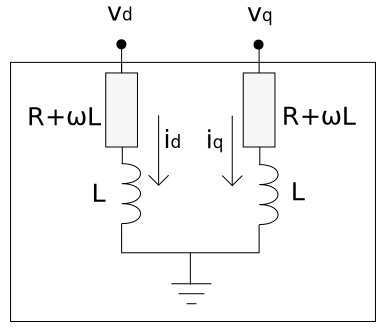
\includegraphics[width=0.5\linewidth]{powersys_load.png}
    \caption{RL Load}
\end{figure}  

Because this model is fully described by LIM atoms, the equations are not given here (see the LIM node atom description in chapter \ref{chap:lim}, figure \ref{fig:lim_dependent_node}).

\section{Transformer-Rectifier Model}

\begin{figure}[h]
    \label{fig:powersys_trload}
    \centering
    \includegraphics[width=0.95\linewidth]{powersys_trload.png}
    \caption{Transformer-Rectifier Load}
\end{figure} 

The Transformer-rectifier load model is based on the model found in \cite{abdelwahed2013}, and includes a non-linear coupling between d and q-axis constant current branches and a dc side with a LIM branch and node. The equivalent circuit model is shown in figure \ref{fig:powersys_trload}. The ac-dc coupling is defined by

\begin{equation} \label{eq:trload_igd}
    i_{gd}=S_{d}i_{dc}   
\end{equation}

\begin{equation} \label{eq:trload_igq}
    i_{gq}=S_{q}i_{dc}   
\end{equation}

\begin{equation} \label{eq:trload_vg}
    v_{g} = \frac{v_{d}}{S_{d}} + \frac{v_{q}}{S_{q}}   
\end{equation}

where the coupling coefficients are

\begin{equation} \label{eq:trload_sd}
    S_{d} = 2 \sqrt{\frac{2}{3}} \frac{\sqrt{3}}{\pi} \cos{\phi}    
\end{equation}

\begin{equation} \label{eq:trload_sq}
    S_{q} = -2 \sqrt{\frac{2}{3}} \frac{\sqrt{3}}{\pi} \sin{\phi}.    
\end{equation}

where $\phi$ is the firing angle. The dc subsystem of this model is a LIM branch, the equations for which are given in chapter \ref{chap:lim}, figure \ref{fig:lim_dependent_branch}.

\section{Synchronous Machine}

The synchronous machine \cite{abdelwahed2013} is modeled at two LIM branches for the electrical model (one for each dq axis), and a LIM node for the mechanical dynamics. The equivalent circuit is shown in figure \ref{fig:powersys_sm}

\begin{figure}[h]
    \label{fig:powersys_sm}
    \centering
    \includegraphics[width=0.95\linewidth]{powersys_sm.png}
    \caption{Synchronous Machine}
\end{figure}

The electro-mechanical dynamics are modeled with the flux differential equations

\begin{equation}
\frac{d}{dt} \psi_{kq} = \frac{r_{kq}}{L_{lkq}} \left( \psi_{kq} - L_{q} i_{qs} - \psi_{q} i_{qs}+L_{ls} i_{qs} \right)
\end{equation}

\begin{equation}
    \frac{d}{dt} \psi_{kd} = \frac{r_{kd}}{L_{lkd}} \left( \psi_{kd} - L_{d} i_{ds} - \psi_{d} i_{ds}+L_{ls} i_{ds} \right)
\end{equation}

\begin{equation}
    \frac{d}{dt} \psi_{fd} = \frac{r_{fd}}{L_{lfdd}} \left( \psi_{fd} - L_{d} i_{ds} - \psi_{d} i_{ds}+L_{ls} i_{ds} - v_{fd} \right)
\end{equation}

where the electrical torque $T_e$ is coupled to the terminal currents $i_{qs}$, $i_{ds}$ as

\begin{equation}
    T_e = \frac{3P}{4} \left( \psi_{ds} i_{qs} - \psi_{qs} i_{ds} \right)
\end{equation}

and the q- and d-axis equivalent fluxes and inductances are given by

\begin{equation}
    L_q = L_{ls} + \frac{L_{mq}L_{lkq}}{L_{lkq} + L_{mq}}
\end{equation}

\begin{equation}
    L_d = L_{ls} + \frac{L_{md} L_{lfd} L_{lkd}}{L_{md} L_{lfd} + L_{md} L_{lkd} + L_{lfd} L_{lkd}}
\end{equation}

\begin{equation}
    \psi_q = \frac{L_{mq}}{L_{mq} + L_{kd}} \psi_kd
\end{equation}

\begin{equation}
    \psi_d = \frac{L_{md} \left( \frac{\psi_{kd}}{L_{lkd}} + \frac{\psi_{fd}}{L_{lfd}} \right) }{1 + \frac{L_{md}}{L_{lfd}} + \frac{L_{md}}{L_{lkd}}}
\end{equation}.

\section{Turbo-Governor Model}

The dynamics of the prime mover and the speed governor are combined into a single model described by

\begin{equation}
    T_m = K_p \delta_r + K_i \theta_r
\end{equation}

where $T_m$ in the mechanical torque, $K_p$ and $K_i$ are the PI controller constants, and the speed deviation $\delta_r$ and rotor angle $\theta_r$ are related to the synchronous speed ($\omega_s$) and the machine rotor speed ($\omega_r$) as

\begin{equation}
    \delta_r = \omega_s - \omega_r
\end{equation}

\begin{equation}
    \frac{d}{dt} \theta = \delta_r.
\end{equation}.

\section{Exciter Model}

The synchronous machine terminal voltage is regulated using an exciter. The exciter model used is a simplified IEEE AC8B Exciter model. This is modeled as four differential equations for three internal signal states as well as the output voltage. 

The input is the per unit terminal voltage magnitude, and the output is the per unit field voltage $v_{fd}$. The differential equations are 

\begin{equation}
    \frac{d}{dt} x_1 = v_{term,pu} - \frac{1}{T_{dr}} x_1
\end{equation}

\begin{equation}
    \frac{d}{dt} x_2 = x_1
\end{equation}

\begin{equation}
    \frac{d}{dt} x_3 = \left( K_{ir} - \frac{K_{dr}}{T^2_{dr}} \right) x_1
    + \frac{K_{ir}}{T_{dr}} x_2 - \frac{1}{T_a} x_3
    + \left( \frac{K_{dr}}{T_{dr}} + K_{pr} \right) v_{term,pu}
\end{equation}

\begin{equation}
    \frac{d}{dt} v_{fd,pu} = \frac{K_a}{T_a T_e} x_3 - \frac{K_e}{T_e} v_{fd,pu}
\end{equation}

where the per unit terminal voltage $v_{t,pu}$ is related to the machine dq quantities and the rated line-line terminal voltage magnitude $V_{base,LL}$ as

\begin{equation}
    v_{term,pu} = \frac{\sqrt{v^2_{qs} + v^2_{ds}}}{V_{base,LL}}
\end{equation}

and the per unit output of the exciter $v_{fd,pu}$ is then scaled by the base voltage $V_{base,LL}$ before being input into to synchronous machine model as

\begin{equation}
    v_{fd} = v_{fd,pu} \cdot V_{base,LL}
\end{equation}.

\section{Induction Machine Model}

The induction machine is modeled as two LIM branches for the electrical model (one for each dq axis) and a LIM node for the mechanical dynamics as shown in figure \ref{fig:powersys_im}

\begin{figure}[h]
    \label{fig:powersys_im}
    \centering
    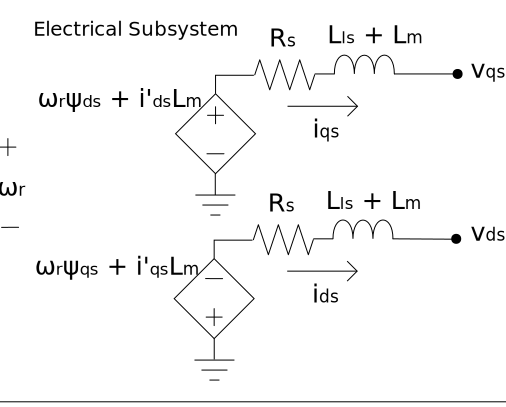
\includegraphics[width=0.95\linewidth]{powersys_im.png}
    \caption{Induction Machine}
\end{figure}

The LIM sources are updated using the flux quantities defined in terms of the instantaneous stator and rotor d- and q- access currents using

\begin{equation}
    \psi_{qs} = L_{ls} i_{qs} + l_m (i_{qs} + i_{qr} )
\end{equation}

\begin{equation}
    \psi_{ds} = L_{ls} i_{ds} + l_m (i_{ds} + i_{dr} )
\end{equation}

\begin{equation}
    \psi_{qr} = L_{lr} i_{qr} + l_m (i_{qr} + i_{qs} )
\end{equation}

\begin{equation}
    \psi_{dr} = L_{lr} i_{dr} + l_m (i_{dr} + i_{ds} )
\end{equation},

And the mechanical dynamics are resolved using the LIM node model in figure \ref{fig:powersys_im}, where the electrical torque $T_e$ is determined from the currents using

\begin{equation}
    T_e = \frac{P}{2J} \left(
    \frac{3P}{4} \left( L_{ls} i_{ds} + L_m
    \left( i_{ds} + i_{dr} \right)\right)
    i_{qs} - \left(L_{ls} i_{qs} + L_m
    \left(i_{qs} + i_{qr} \right)\right)
    i_{ds}-T_b \left( \frac{\omega_r}{\omega_s}
    \right)^3 \right)
\end{equation}

where $P$ is the number of pole pairs, $T_b$ is the base torque, and $\omega_s$ and $\omega_r$ are the synchronous and rotor speeds respectively. 

\section{Simulation Scenario and Benchmark Solution}

In the simulation scenario, the system starts in steady-state (all state derivatives are zero), using a standard iterative ODE operating point solution. At time $t=0$ seconds, the active power of RL load is increased by 20\%. A reference solution (denoted "ODE" in the output plots) is run with identical parameters and events to compare the results and quantify error. 

In order to provide results for performing accuracy and performance bench-marking, a traditional integration method was used that is well-suited to non-linear, stiff systems. The modeling method used to benchmark accuracy  and performance uses a representation of the system as a set of non-linear, first order differential equations. The QDL formulation of the power system provides a full state-space description of the system, including the system Jacobian matrix that can be used directly with many numerical integration techniques. The integration method used to compute the benchmark is an implicit Runge-Kutta method of the Radau IIA family of order 5, a method well-suited for these types of stiff systems. The fixed time step was chosen to be $10 \mu s$ to easily accommodate the fastest eigenvalues of the system.

\section{Simulation Results}

Each plot presented for the simulation results includes the QDL results as the solid color curves, the benchmark results as a dashed gray curve, and the cumulative atom updates as a dashed color curve with a separated $y$ axis on the right. Each plotted atoms' results are shown for the entire 60 seconds of simulation, along with zoom plots to the transient around the disturbance at 1 second simulation time. The time range of each zoom plot is chosen to highlight the performance of QDL for the specific dynamic behavior for that specific state, as some states move much faster than others. Some plots included filtered results to reduce spurious noise as discussed in section \ref{sec:filtering}.

\begin{figure}[h]
    \centering
    \includegraphics[width=0.95\linewidth]{powersys_plot_loadinc_sm_wr.png}
    \caption{Synchronous machine speed.}
    \label{fig:powersys_plot_loadinc_sm_wr}
\end{figure}

\begin{figure}[h]
    \centering
    \includegraphics[width=0.95\linewidth]{powersys_plot_loadinc_sm_wr_ZOOM.png}
    \caption{Synchronous machine speed, zoom to transient.}
    \label{fig:powersys_plot_loadinc_sm_wr_ZOOM}
\end{figure}

\begin{figure}[h]
    \centering
    \includegraphics[width=0.95\linewidth]{powersys_plot_loadinc_sm_iqs.png}
    \caption{Synchronous machine q-axis stator current (filtered, $fc=100 Hz$).}
    \label{fig:powersys_plot_loadinc_sm_iqs}
\end{figure}

\begin{figure}[h]
    \centering
    \includegraphics[width=0.95\linewidth]{powersys_plot_loadinc_sm_iqs_ZOOM.png}
    \caption{Synchronous machine q-axis stator current, zoom to transient (filtered, $fc=100 Hz$)}
    \label{fig:powersys_plot_loadinc_sm_iqs_ZOOM}
\end{figure}

\begin{figure}[h]
    \centering
    \includegraphics[width=0.95\linewidth]{powersys_plot_loadinc_rlload.png}
    \caption{RL Load currents.}
    \label{fig:powersys_plot_loadinc_rlload}
\end{figure}

\begin{figure}[h]
    \centering
    \includegraphics[width=0.95\linewidth]{powersys_plot_loadinc_rlload_ZOOM.png}
    \caption{RL Load currents, zoom to transient.}
    \label{fig:powersys_plot_loadinc_rlload_ZOOM}
\end{figure}

\begin{figure}[h]
    \centering
    \includegraphics[width=0.95\linewidth]{powersys_plot_loadinc_trload.png}
    \caption{Transformer-rectifier load d-axis current and dc voltage.}
    \label{fig:powersys_plot_loadinc_trload}
\end{figure}

\begin{figure}[h]
    \centering
    \includegraphics[width=0.95\linewidth]{powersys_plot_loadinc_trload_ZOOM.png}
    \caption{Transformer-rectifier load d-axis current and dc voltage, zoom to transient.}
    \label{fig:powersys_plot_loadinc_trload_ZOOM}
\end{figure}

\begin{figure}[h]
    \centering
    \includegraphics[width=0.95\linewidth]{powersys_plot_loadinc_bus1_vd.png}
    \caption{Bus 1 d-axis voltage.}
    \label{fig:powersys_plot_loadinc_bus1_vd}
\end{figure}

\begin{figure}[h]
    \centering
    \includegraphics[width=0.95\linewidth]{powersys_plot_loadinc_bus1_vd_ZOOM.png}
    \caption{Bus 1 d-axis voltage, zoom to transient.}
    \label{fig:powersys_plot_loadinc_bus1_vd_ZOOM}
\end{figure}

\begin{figure}[h]
    \centering
    \includegraphics[width=0.95\linewidth]{powersys_plot_loadinc_im_wr.png}
    \caption{Induction machine speed.}
    \label{fig:powersys_plot_loadinc_im_wr}
\end{figure}

\begin{figure}[h]
    \centering
    \includegraphics[width=0.95\linewidth]{powersys_plot_loadinc_im_wr_ZOOM.png}
    \caption{Induction machine speed, zoom to transient.}
    \label{fig:powersys_plot_loadinc_im_wr_ZOOM}
\end{figure}

\begin{figure}[h]
    \centering
    \includegraphics[width=0.95\linewidth]{powersys_plot_loadinc_cable23_100hz.png}
    \caption{Cable currents from bus 2 to bus 3 q-axis (filtered, $f_c=100 Hz$).}
    \label{fig:powersys_plot_loadinc_cable23_100hz}
\end{figure}

\begin{figure}[h]
    \centering
    \includegraphics[width=0.95\linewidth]{powersys_plot_loadinc_cable23_ZOOM_100hz.png}
    \caption{Cable currents from bus 2 to bus 3 q-axis, zoom to transient (filtered, $f_c=100 Hz$).}
    \label{fig:powersys_plot_loadinc_cable23_ZOOM_100hz}
\end{figure}

From inspection of the plots in figures \ref{fig:powersys_plot_loadinc_sm_wr} to \ref{fig:powersys_plot_loadinc_cable23_ZOOM_100hz}, the transient behavior of all states tracts the benchmark solution very well. The steady-state behavior, although bounded, shows significant oscillations. This highlights the importance of the topics discussed in chapter \ref{chap:steadystate} for detecting steady-state, and filtering spurious oscillations from the results using post-simulation filtering.  
 
\section{Error Analysis}

Error was quantified using the normalized RMS deviation calculation defined as

\begin{equation}
    \text{NRMSD} = \frac{ \sqrt{ \frac{\sum_{i=1}^N{(y_i - q_i)^2}}{N} } }{\max{y} - \min{y}}.
\end{equation}

where $y_i$ is the benchmark (ODE) solution result for the state variable at point i, $q_i$ is the quantized QDL solution result for the state variable at point i, $N$ is the number of solution points, and the quantity $\max{y} - \min{y}$ is the dynamic range of the variable in the benchmark simulation. 
    
This method of producing aggregated error values was chosen in order to provide error results that could be meaningfully compared across the states of the simulation, given the vastly different offsets and dynamic ranges between the states. The errors observed for the load increase simulation are shown in the sorted bar chart in figure \ref{fig:powersys_plot_error}.

\begin{figure}[h]
    \centering
    \includegraphics[width=0.95\linewidth]{powersys_plot_error.png}
    \caption{Simulation NRMSD error by state variable}
    \label{fig:powersys_plot_error}
\end{figure}

The q-axis current on the cable from bus 2 to 3 is the state with the highest aggregated error in the simulation. This is not surprising given the level of high-amplitude noise seen in the simulation output for this variable. See chapter \ref{chap:steadystate} for further discussion on post-process filtering of these data to improve readability of results, and to reduce error.

\section{Performance Analysis}

To analyze the performance of the QDL method for this system, a proxy for computation intensity was used to estimate the relative performance of the QDL method against the benchmark ODE solution. This proxy is the cumulative number of updates for each atom. Although not directly comparable to time-slicing method time step counts, it gives us a good approximation of the relative computational efficiency of the QDL method vs. the reference ODE solution. Note that, in order to produce a stable simulation, a time step of $10\mu s$ was used, which results in $6 \times 10^{5}$ time steps for a 60 second (simulation time) simulation.  

\begin{figure}[h]
    \centering
    \includegraphics[width=0.75\linewidth]{powersys_vref_inc_updates_60s_sm.png}
    \caption{Cumulative QDL atom updates vs. simulation time, synchronous machine states}
    \label{fig:powersys_vref_inc_updates_60s_sm}
\end{figure} 

\begin{figure}[h]
    \centering
    \includegraphics[width=0.75\linewidth]{powersys_vref_inc_updates_60s_im.png}
    \caption{Cumulative QDL atom updates vs. simulation time, induction machine states}
    \label{fig:powersys_vref_inc_updates_60s_im}
\end{figure} 

The key result shown in the plot in figures \ref{fig:powersys_vref_inc_updates_60s_sm} and \ref{fig:powersys_vref_inc_updates_60s_im} is that the cumulative updates of the QDL atom states are less frequent than the required ODE benchmark solution time steps, in some cases by several orders of magnitude. Also, in the case of some states, such as the synchronous machine mechanical quantities (the rotor speed $\omega_r$ and rotor angle $\theta$), the trajectories of the cumulative curves become very flat, meaning there are very few updates needed for these states at steady-state.

Because the accuracy and computational intensity are related to the chosen quantization step size in QSS-based integration methods (a trade-off that does not exist with traditional methods), these metrics are difficult to compare directly. Also, different quantization step sizes were selected for each QDL atom state based on the dynamic range of each variable in the simulation scenarios. With the selected quantization step sizes, the simulation results are accurate to within a relative error of $\pm 5\%$ relative to the reference simulation (a 5th order Implicit Runge-Kutta algorithm with a fixed time step of $10 \mu s$). Also, the proxy metrics for computational intensity (the number of state updates for the QSS solution, and the number of time steps for the reference solution) show that the theoretical performance of fully optimized code would result in faster performance for the QDL versus the reference simulation.